\section{The \Commonalities Language}
\label{chap:language:commonalities}

\mnote{Section overview}
In this section, we present an overview of the \commonalities language.
It constitutes one possible realization of a language for the \commonalities approach with the conceptual design choices that we have discussed in the previous section.
This especially includes an internal specification of concepts.
To give an impression of the language, we first introduce two examples for specifications in a prototypical realization of the language with a textual syntax, which we have already proposed in previous work~\owncite{klare2019models} and which was originally developed in the bachelor's thesis of \textowncite{gleitze2017a} and extended in the master's thesis of \textowncite{hennig2020ma}.
We then give an overview of the language elements and introduce their general semantics before explaining the different categories of them at the given examples.
Since we focus on the language concepts, we refer for details on its realization with a textual syntax to the theses of \textowncite{gleitze2017a} and \textowncite{hennig2020ma}.


\subsection{Examples in Textual Syntax}

\lstinputlisting[language=commonalities, float,
    caption={[Exemplary \commonality for clases]An exemplary specification for an extract of the \texttt{Class} \commonality between \gls{UML} and Java in the \commonalities language.},
    captionpos=b,
    label=lst:language:class_example,
]{listings/quality/language/class_example.lst}

\lstinputlisting[language=commonalities, float,
    caption={[Exemplary \commonality for components]An exemplary specification for an extract of the \texttt{Component} \commonality between \gls{PCM}, UML and the object-oriented design \conceptmetamodel in the \commonalities language.},
    captionpos=b,
    label=lst:language:component_example,
]{listings/quality/language/component_example.lst}

\mnote{Examples overview}
We depict two examples for specifications in our prototype of the \commonalities language with a textual syntax in \autoref{lst:language:class_example} and \autoref{lst:language:component_example}.
The specifications depict extracts of a \commonality for classes in \gls{UML} and Java, as well as extracts of a \commonality for components in \gls{PCM}, \gls{UML} and classes with their containing packages in the object-oriented design \conceptmetamodel.
The extracts are selected to reflect the different elements of the \commonalities language without introducing unnecessary complexity.
We sketch the meaning of the examples in the following and clarify them along with the subsequent introduction of the language elements more precisely.

\mnote{Class \commonality example}
The class \commonality, depicted in \autoref{lst:language:class_example}, is restricted to their names and methods.
In \gls{UML}, a class is represented by a class that is contained in a unique instance of a \gls{UML} model.
In Java, a class is also represented by a class that is contained in a compilation unit, which depicts one file consisting of imports and class specifications as a single unit of compilation~\cite{heidenreich2009jamopp-report}.
Names are represented equally in \gls{UML} and Java classes.
The name of the compilation unit is defined by the fully qualified name of the class, i.e., the concatenation of its namespace and the class name separated by a dot.
The specification expresses this as the class name to be the suffix of the compilation unit name after the namespace followed by a dot.
Methods are specified in a dedicated \commonality in the object-oriented design \conceptmetamodel, such that they are only referenced in the class \commonality, but without any specification of the relations of their contents.

\mnote{Component \commonality example}
The component \commonality, depicted in \autoref{lst:language:component_example}, is restricted to their names.
In \gls{PCM} and \gls{UML}, components are realized by explicit component or basic component \metaclasses, respectively, which share the same name.
In object-oriented design, components are defined to be represented by classes contained in a package.
Classes are only considered to represent components when their name has an \enquote{Impl} suffix and their name is then defined to be the component name with an \enquote{Impl} suffix.
The specification defines this as a prefix, analogous to the suffix for the name of a compilation unit, as it denotes that the component name is the prefix of the class name before \enquote{Impl}.
Finally, the package name is defined to be the component name but starting with a lowercase letter whereas the component name start is defined to start with an uppercase letter.
Analogous to the prefix definition for the class name, the specification defines a \texttt{firstUpper} operation as the component name shall be the package name with the first letter in uppercase.


\subsection{Elements Overview}

\mnote{Categories of elements}
The \commonalities language essentially consists of three categories of elements.
First, at a top level the structure of \commonalities needs to be defined in terms of specifying for each of them the \conceptmetamodels they belong to, as well as the features in terms of attributes and references it describes.
Second, each \commonality needs to define its manifestations, i.e., the \metaclasses of \concretemetamodels or other \conceptmetamodels being its manifestations, along with conditions defining when instances of \metaclasses are to be considered a manifestation.
This defines when a manifestation relation between a \commonality and \metaclasses of another \conceptmetamodel or \concretemetamodel exist.
Third, each \commonality needs to define the relations of its features to those of its manifestations.
This defines the manifestation relations, i.e., the conditions that have to hold for considering a manifestation consistent to a \commonality.

\begin{figure}
    \centering
    \newcommand{\hdistance}{7.6em}
\newcommand{\classwidth}{5.5em}
\newcommand{\vdistance}{5em}

\begin{tikzpicture}[
    existing/.style={fill=lightgray!20}
]

\umlclassvarwidth[, existing]{metamodel}{}{Metamodel}{
name : String\\
}{\classwidth} 

\umlclassvarwidth[, existing, right=\hdistance of metamodel.north, anchor=north]{class}{}{Class}{
name : String\\
}{\classwidth}  

\umlclassvarwidth[, existing, right=\hdistance of class.north, anchor=north]{reference}{}{Reference}{
name : String\\
}{\classwidth}

\umlclassvarwidth[, existing, right=\hdistance of reference.north, anchor=north]{attribute}{}{Attribute}{
name : String\\
}{\classwidth}

\umlclassvarwidth[, below=\vdistance of metamodel.north, anchor=north]{concept}{}{Concept}{
}{\classwidth}  

\umlclassvarwidth[, right=\hdistance of concept.north, anchor=north]{commonality}{}{Commonality}{
root : Boolean\\
}{\classwidth}

\umlclassvarwidth[, below=\vdistance of commonality.north, anchor=north]{manifestation}{}{Manifestation}{
}{\classwidth} 

\umlclassvarwidth[, right=\hdistance of manifestation.north, anchor=north]{commonality_reference}{}{Commonality\\Reference}{
}{\classwidth}

\umlclassvarwidth[, right=\hdistance of commonality_reference.north, anchor=north]{commonality_attribute}{}{Commonality\\Attribute}{
}{\classwidth}


\umlclassvarwidth[, below left=\vdistance and \hdistance of manifestation.north, anchor=north]{manifestation_class}{}{Manifestation\\Class}{
alias : String\\
single : Boolean\\
}{\classwidth}

\umlclassvarwidth[, below=\vdistance of manifestation.north, anchor=north]{manifestation_condition}{}{Manifestation\\Condition}{
dir : Direction\\
}{\classwidth}

\umlclassvarwidth[, below=\vdistance of commonality_attribute.north, anchor=north]{attribute_relation}{}{Attribute\\Relation}{
dir : Direction\\
}{\classwidth} 

\umlclassvarwidth[, below=\vdistance of commonality_reference.north, anchor=north]{reference_relation}{}{Reference\\Relation}{
dir : Direction\\
}{\classwidth} 

\umlclassvarwidth[, below=\vdistance of manifestation_condition.north, anchor=north]{manifestation_operator}{}{Manifestation\\Operator}{
}{\classwidth}

\umlclassvarwidth[, below=\vdistance of attribute_relation.north, anchor=north]{attribute_operator}{}{Attribute\\Operator}{
}{\classwidth} 

\umlclassvarwidth[, below=\vdistance of reference_relation.north, anchor=north]{reference_operator}{}{Reference\\Operator}{
}{\classwidth} 

\umlclassvarwidth[, below=\vdistance of reference_operator.north, anchor=north]{operand}{}{\textit{Operand}}{
}{\classwidth}

\umlclassvarwidth[, below left=\vdistance and \hdistance of operand.north, anchor=north]{manifestation_operand}{}{\textit{Manifestation}\\\textit{Operand}}{
}{\classwidth}

\umlclassvarwidth[, below right=\vdistance and 0em of operand.north, anchor=north]{literal_operand}{}{Literal\\Operand}{
}{\classwidth}

\umlclassvarwidth[, right=\hdistance of literal_operand.center, anchor=center]{direction}{}{\umlenumlabel\\Direction}{
\itshape
Bidirectional\\
Checkonly\\
Enforce\\
}{\classwidth}

\umlclassvarwidth[, below left=\vdistance and \hdistance of manifestation_operand.north, anchor=north]{manifestation_class_operand}{}{Manifestation\\Class\\Operand}{
}{\classwidth}

\umlclassvarwidth[, below left=\vdistance and 0em of manifestation_operand.north, anchor=north]{manifestation_attribute_operand}{}{Manifestation\\Attribute\\Operand}{
}{\classwidth}

\umlclassvarwidth[, below right=\vdistance and \hdistance of manifestation_operand.north, anchor=north]{manifestation_reference_operand}{}{Manifestation\\Reference\\Operand}{
}{\classwidth}


% INHERITANCE
\umlsubclassof{concept}{--}{metamodel}
\umlsubclassof{commonality}{--}{class}
\umlsubclassof{commonality_attribute}{--}{attribute}
\umlsubclassof{commonality_reference}{--}{reference}

\umlsubclassof{manifestation_operand}{|- ([yshift=-1.5em]operand.south) --}{operand}
\draw (literal_operand) |- ([yshift=-1.5em]operand.south);

\umlsubclassof{manifestation_class_operand}{|- ($(manifestation_attribute_operand.north)!0.5!(manifestation_operand.south)$) --}{manifestation_operand}
\draw (manifestation_attribute_operand) -- ($(manifestation_attribute_operand.north)!0.5!(manifestation_operand.south)$);
\draw (manifestation_reference_operand) |- ($(manifestation_attribute_operand.north)!0.5!(manifestation_operand.south)$);

% REFERENCES
%\umlassociationfromto{(class) -- node[uml cardinality end, pos=1, above right] {1} (metamodel)}
\umlcomposition{(metamodel.east) -- node[uml cardinality end, pos=1, above left] {*} (class.west|-metamodel.west)}
\umlcomposition{(concept.east) -- node[uml cardinality end, pos=1, above left] {*} (commonality.west|-concept.west)}
\umlcomposition{(class.east) -- node[uml cardinality end, pos=1, above left] {*} (reference.west|-class.east)}
\umlcomposition{([xshift=1em]class.north) -- ++(0,1em) -| node[uml cardinality end, pos=1, above right] {*} (attribute.north)}

\umlcomposition{(commonality) -- node[uml cardinality end, pos=1, above right] {*} (manifestation)}
\umlcomposition{([xshift=-1em]commonality.south east) -- ++(0,-1em) -|node[uml cardinality end, pos=1, above right] {*} ([xshift=1em]commonality_reference.north west)}
\umlcomposition{([yshift=0.5em]commonality.east) -| node[uml cardinality end, pos=1, above left] {*} ([xshift=-1.5em]commonality_attribute.north)}

\umlassociationfromto{([xshift=-1em]commonality_reference.north) |- node[uml cardinality end, pos=1, above right] {1} node[uml role end, pos=1, below right] {type} ([yshift=-1em]commonality.east)}

\umlcomposition{([xshift=1em]manifestation.south west) -- ++(0,-1.5em) -| node[uml cardinality end, pos=1, above left] {1..*} ([xshift=-1em]manifestation_class.north east)}
\umlcomposition{(manifestation) -- node[uml cardinality end, pos=1, above left] {*} (manifestation_condition)}
\umlcomposition{(commonality_attribute) -- node[uml cardinality end, pos=1, above left] {*} (attribute_relation)}
\umlcomposition{(commonality_reference) -- node[uml cardinality end, pos=1, above left] {*} (reference_relation)}

\umlaggregation{(manifestation_condition) -- node[uml cardinality end, pos=1, above left] {*} (manifestation_operator)}
\umlaggregation{(attribute_relation) -- node[uml cardinality end, pos=1, above left] {*} (attribute_operator)}
\umlaggregation{(reference_relation) -- node[uml cardinality end, pos=1, above left] {*} (reference_operator)}

\umlaggregation{([xshift=1em]manifestation_class.north west) |- node[uml cardinality start, pos=0, above right] {*} ++(-1.5em,\vdistance) |- ([xshift=-1em,yshift=1em]class.north) -- node[uml cardinality end, pos=1, above left] {1} ([xshift=-1em]class.north)}

\umlcomposition{(attribute_relation.west) -- ++(-0.8em,0) |- node[uml cardinality end, pos=1, below right] {*} (operand.east)}
\umlcomposition{(reference_relation.west) -- ++(-0.8em,0) |- node[uml cardinality end, pos=1, above left] {*} ([yshift=0.8em]operand.west)}
\umlcomposition{([yshift=-0.5em]manifestation_condition.west) -- ++(-0.8em,0) |- node[uml cardinality end, pos=1, above left] {*} node[uml cardinality end, pos=1, below left] {rightOperand} ([yshift=-0.8em]operand.west)}
\umlcomposition{([yshift=0.5em]manifestation_condition.west) -- ++(-1.1em,0) |- node[uml cardinality end, pos=1, above left] {*} node[uml cardinality end, pos=1, below left] {leftOperand} ([yshift=0.8em]manifestation_operand.west)}

\umlassociationfromto{([yshift=-0.8em]manifestation_operand.west) -| node[uml cardinality end, pos=1, below right] {1} ([xshift=-1em]manifestation_class.south)}
\umlassociationfromto{(manifestation_attribute_operand.south) -- ++(0,-0.8em) -| ([xshift=0.8em, yshift=-1.2em]attribute.south east) -| node[uml cardinality end, pos=1, below right] {1} ([xshift=1.5em]attribute.south)}
\umlassociationfromto{(manifestation_reference_operand.east) -| ([xshift=0.4em, yshift=-2em]attribute.south east) -| node[uml cardinality end, pos=1, below right] {1} ([xshift=1.5em]reference.south)}

\end{tikzpicture}
    \caption[\commonalities language elements]{Class diagram with the essential elements of the \commonalities language and their relations. Elements that exist independent from the language are depicted in the top row.}
    \label{fig:language:elements}
\end{figure}

\mnote{Structural elements}
\autoref{fig:language:elements} depicts the essential elements of the \commonalities language.
At the top, it depicts \emph{metamodels}, \emph{\metaclasses}, \emph{references} and \emph{attributes} as already existing in the notion of a general modeling formalism and as specified in \concretemetamodels.
The language introduces \emph{concepts}, which represent the \conceptmetamodels, and \emph{\commonalities}, of which such a concept consists.
In our realization, they can be considered specializations of metamodels and \metaclasses but with the special semantics of being only auxiliary artifacts for the \commonalities approach.
A \commonality consists of \emph{\commonality references} and \emph{attributes}, which, again, can be considered specializations of ordinary references and attributes.
In the given examples, we have attributes for names and a reference to methods.
Additionally, a \commonality contains \emph{manifestations}.
Each manifestation represents the realization of the concept represented by the \commonality in another metamodel by one or more  \metaclasses and potentially further conditions for them.
Such manifestation are, for example, a class and a compilation unit in Java for the class \commonality depicted in \autoref{lst:language:class_example}.
In preparatory work~\owncite{gleitze2017a,hennig2020ma}, as well as in the current state of prototypical implementation of the language~\owncite{vitruvFrameworkGithub}, such manifestations have also been called \emph{participations}.
Each \commonality reference and attribute is complemented by \emph{reference} and \emph{attribute relations} that define how these features are related to information in the manifestations.

\mnote{Relational elements}
In consequence, the manifestation conditions together with the attribute and reference relations define the consistency relations between the \commonality and its manifestations, which we have introduced as manifestation relations.
All these relations consists of \emph{operators}, which define how elements are related, and \emph{operands}, which define the involved elements to be considered by the operator. 
The operators can be considered specifications of transformation rules, which take operands providing the information necessary to check or preserve consistency.
In our language realization, operators can be specified by implementing specific interfaces of an \gls{API} and thus dynamically extending the language with arbitrary operators.
In consequence, these operators can be treated as reusable libraries containing operators at different levels of abstraction.
They can, however, also be defined as a static part of the language and thus without the possibility to extend them.
Operators have a \emph{direction}, as they may enforce the defined relation either in both directions or only in one of them.
For example, the name of a class in \autoref{lst:language:class_example} is related to the Java class name bidirectionally (denoted by \enquote{=}).
In consequence, a change of the Java class name leads to the change of the name of the class \commonality, which then changes the \gls{UML} class name, but also a change of the class \commonality name, e.g., because of a change of the \gls{UML} class name, leads to a change of the Java class name.
The name of a compilation unit, however, is only enforced, because it is derived from the Java class name, such that a change is propagated because of the changed Java class name anyway.

\mnote{Simplifications}
For reasons of simplicity, we omitted several elements of the language realization, which concerns generalizations as well as specializations of the depicted elements.
For example, manifestation conditions, reference and attribute relations represent relations between the \commonality and its manifestations, especially comprising a direction, which can be represented in a \texttt{Relation} supertype.
Likewise, the three operator types for manifestations, references and attributes can be derived from a common \texttt{Operator} supertype.


\subsection{Language and Elements Semantics}

\mnote{Consistency relations by \commonalities}
A \commonality defines the elements that different manifestations have in common and how they are related.
For example, the class \commonality given in \autoref{lst:language:class_example} denotes that classes have names and methods in common and that they are related by specific naming schemes of name attributes and specific references containing representations of methods.
Thus, whenever there are elements in one model that match one of the specifications for a manifestation in terms of instantiating the defined classes and fulfilling the defined conditions, there must be elements in other models matching the other manifestation specifications and fulling the defined relations for attributes and references.
In theory, from such a specification consistency relations, according to \autoref{def:consistencyrelation}, could be derived, which enumerate the tuples of instances of the \metaclasses in the manifestations that fulfill the manifestation conditions, as well as the attribute and reference relations.

\mnote{Consistency preservation}
We especially want to preserve consistency rather than only checking it and thus derive consistency preservation rules from such a specification.
In \autoref{chap:language:commonalities:operationalization}, we discuss such an operationalization in more detail.
In general, we distinguish the instantiation, update and deletion of a \commonality, according to the scenarios already depicted for \mappings in the bidirectional \mappings language~\cite[Sec. 7.2.1]{klare2020Vitruv-JSS}.
The \commonalities language specifies a bidirectional transformation between a \commonality and each of its manifestations.
Thus the behavior of each such transformation conforms to the behavior of the \mappings language, in which we could define the transformation between a \commonality and its manifestation.

\begin{properdescription}
\item[Instantiation:] \mnote{\Commonality instantiation}
A \commonality is \emph{instantiated}, whenever elements are added to a model such that they instantiate the \metaclasses of a manifestation of that \commonality and fulfill the defined manifestation conditions.
We say that these elements \emph{match} the manifestation of the \commonality.
In that case, an instance of the \metaclass realizing the \commonality is created and its attributes and references are initialized with values according to the relations defined in the \commonality.
Then, for each other manifestation, instances of the \metaclasses are generated and inserted into a model according to the specified manifestation conditions and defined relations of attributes and references.
For example, according to \autoref{lst:language:component_example}, whenever a Java class with the suffix \enquote{Impl} is created and inserted into a package, a component \commonality with the name of the class without that suffix is created, and a basic component in \gls{PCM}, as well as a component in \gls{UML} with that name are created.

\item[Deletion:] \mnote{\Commonality deletion}
A \commonality is \emph{deleted} whenever the elements, for which a \commonality was instantiated, do not match the manifestation anymore.
Then, the instance of the \metaclass realizing the \commonality is removed, as well as the instantiations of all \metaclasses of the other manifestations.
For example, whenever a Java class representing a component is removed, or even if only the \enquote{Impl} suffix is removed, the \commonality and all other manifestations in \gls{PCM} and \gls{UML} are removed.

\item[Update:] \mnote{\Commonality update}
A \commonality is \emph{updated} whenever any of the attribute or reference values of the elements of a manifestation, for which a \commonality was instantiated, gets changed.
In that case, the values in the \commonality and all other manifestations are updated if the changed value is used in the according attribute or reference relations, i.e., if it is one of its operands.
The relation also defines a direction to indicate whether the change is only checked in the manifestation, i.e., whether a change of any value in the manifestation leads to an update of the value in the \commonality and the other manifestations, whether the change is only enforced, i.e., whether a change of a value of the \commonality leads to a change of the values in the manifestation, or whether it is bidirectional, i.e., both checked and enforced.
This ensures that consistency is preserved for the elements for which a \commonality is instantiated.
\end{properdescription}

\mnote{Relation to \mappings language}
While for the instantiation and deletion of a \commonality only the manifestation classes and their conditions are relevant, for an update only the attribute and reference relations are relevant.
To relate this to the \mappings language, manifestations and their conditions conform to \emph{single-sided conditions}, whereas attribute and reference relations conform to \emph{bidirectionalizable conditions} of \mappings~\cite[Sec. 7.2.1]{klare2020Vitruv-JSS}.
Since a \commonalities specification can be seen as a combination of defining multiple \mappings in the \mappings language, large parts of the semantics and possibilities for the realization are comparable.
We thus focus on the structure that \commonalities define on top of bidirectional mappings and explicitly refer to work on \mappings for concepts that have already been researched and are reusable, such as operators and methods to define and execute them bidirectionally.

\mnote{Alignment with consistency relations}
In \autoref{chap:synchronization:gap:alignment}, we have also discussed the addition, removal and change of condition elements as the relevant change types to be distinguished when realizing consistency preservation.
This conforms to the scenarios of instantiation, deletion and update of a \commonality.
The addition of a condition element of a consistency relations defined by a \commonality specification means that the according manifestation is matched and thus the \commonality is instantiated.
The removal and update conform to the deletion and update of a \commonality analogously.


\subsection{\Commonalities and Manifestations}

\mnote{\Commonalities and concepts}
The top-level elements of the \commonalities language are \commonalities.
Each of them depicts a common concept, such as a class or a component, and is associated with a \conceptmetamodel, which groups common concepts that belong together.
In the given examples, each specification contains one \commonality and starts with a specification of the \conceptmetamodel it belongs to, comparable to a package specification of a class in Java.
These \conceptmetamodels are named \emph{ObjectOrientedDesign} and \emph{ComponentBasedDesign}, according to the ones we have proposed in the examples for composing \commonalities in \autoref{chap:improvement:commonalities:composition}.

\mnote{Manifestations and their classes}
The specification of each \commonality starts with its manifestations, which are \metaclass tuples of the \concretemetamodels or \conceptmetamodels in which the \commonality manifests, together with further conditions on when instances of these \metaclasses form a manifestation of a common concept.
Such a manifestation denotes which elements have to exist in a model and which conditions they have to fulfill to consider these elements a manifestation of a common concept described by the \commonality.
The \metaclass tuples are represented by \emph{manifestation classes}, which only reference an ordinary \metaclass, but may also have an alias for referencing it.
The \metaclass they reference can be an ordinary class of a \concretemetamodels, such as \gls{UML} components in \autoref{lst:language:component_example}, or they may be \commonalities of a \conceptmetamodel, such as classes in object-oriented design in \autoref{lst:language:class_example}.

\mnote{Single manifestation classes}
Additionally, manifestation classes can be declared \emph{single} to denote that they only occur uniquely within one metamodel and do not share a \commonality with others, comparable to a singleton, but are still relevant for the \commonalities specification.
For example, a \gls{UML} model always has a root container of the \metaclass \emph{Model}, which does not share a \commonality with Java in the object-oriented design \conceptmetamodel and exists uniquely, as there may only be one such \gls{UML} model.
An alternative representation of such elements that need to uniquely exist in one of the manifestations but are not represented in others would be \commonalities with only one manifestation that are bootstrapped.
This means that such a \commonality and its manifestation would always exist and is thus created as soon as the development of a system is started rather than instantiating it when a manifestation is matched.
For example, a \gls{UML} model would be created as soon as a new software development project is started.
\citeauthor{kramer2017a} uses such a bootstrap representation of elements in his \mappings language for bidirectional transformations~\cite[Sec. 7.1]{kramer2017a}.

\mnote{Manifestation conditions}
Manifestations further define manifestation conditions, which specify when instances of the \metaclasses referenced by the manifestation classes shall be considered a manifestation of the defined \commonality.
Obviously, not every instance tuple shall be considered as such.
This can further depend on properties of the single objects or on the relation between them.
For example, for the manifestation of components in object-oriented design according to \autoref{lst:language:component_example}, only classes matching a specific naming scheme shall be considered components, and only a pair of class and package in which the class is contained in that package shall be considered a component, but not any pair in which the class is not contained in the package at all.
Such conditions can be seen as restrictions at the instance or model level, whereas the \metaclass tuples define a restriction at the type or metamodel level.

\mnote{Manifestation Operators}
A manifestation condition consists of a \emph{manifestation operator}, a \emph{left operand} and a list of \emph{right operands}.
The left operand can be considered the reference element of the operator. 
It can be any \metaclass of the manifestation or any of its attributes or references, for which a condition shall be defined.
The operator can be any Boolean-valued condition that is evaluated for the left operand and potentially further right operands, which can, again, be \metaclasses of the manifestation or any of their features, or a literal, such as a fixed number or string.
\autoref{lst:language:component_example} contains the operator \emph{in}, which validates whether the value of the left operand is contained within a reference given as the right operand.
In addition, the operator \emph{hasSuffix} checks whether the value of the left operand contains the right operand as a suffix.


\subsection{Features and Relations}
\label{chap:language:commonalities:features}

\mnote{\Commonality attributes and references}
In addition to manifestations, a \commonality defines features, i.e., attributes and references, which represent the information shared by several manifestations, as well as their relations to information defined in the manifestations.
Attributes only need to be identifiable by a name, whereas references, in addition, need to define the type they reference.
This type has to be a \commonality again, such as the methods reference of a class referencing the \commonality \texttt{ObjectOrientedDesign:ClassMethod} in \autoref{lst:language:class_example}.

\mnote{Attribute and reference relations}
While these attributes and references only define the structure of the \commonality, the relations defined within them express how attributes and references are represented in the manifestations.
Reference and attribute relations consist of an operator and operands.
The operator defines how the \commonality attribute or reference is related to features of the manifestations or other literal values, which are passed to the operator as operands.
For example, the name attribute of the component \commonality in \autoref{lst:language:component_example} is related to the name of a class in object-oriented design by a \emph{prefix} operator, which takes the class name and an \enquote{Impl} string as operands.
That operator expresses that the name of the component \commonality is the prefix of the given class name removing \enquote{Impl}.

\mnote{Operands and direction of relations}
In comparison to manifestation conditions, attribute and reference relations only have one set of operands, because the element for which the relation is defined is implicitly given by the \commonality attribute or reference, whereas a manifestation condition must explicitly define which \metaclass or feature it belongs to.
Analogous to manifestation conditions, they do, however, define a direction.
For example, in \autoref{lst:language:component_example}, the relation between the name of the component \commonality and the name of the class in object-oriented design is defined to be bidirectional (denoted with a \enquote{=}), which means that changes of both elements are propagated to the other.
The component name is also related to the package name, in which the class in object-oriented design is contained.
This relation is, however, defined as an \emph{enforce} relation, such that the package name is enforced whenever the name of the component changes, but a modification of the package name does not lead to any changes of the component name.

\lstinputlisting[language=Java, float,
    caption={[Implementation of a prefix operator for \commonalities]An implementation of the prefix operator for \commonalities as used in the prototypical implementation of the \commonalities language. The operator is derived from an abstract implementation for operators relating attributes to attributes. The generic type parameters denote the attribute types in the \commonality as well as in the manifestation. Adapted from the \vitruv code repository~\owncite{vitruvCBSEGithub}.},
    captionpos=b,
    label=lst:language:prefix_operator,
]{listings/quality/language/prefix_operator.lst}

\mnote{Implementation of operators}
Whenever a relation is defined as bidirectional, the operator needs to define how changes are propagated in both directions, i.e., how to update the \commonality attribute or reference among changes in any of the operands and how to update the operands whenever the \commonality attribute or reference is changed.
Our prototypical implementation allows to define such operators in Java code.
They need to be derived from a common interface to dynamically extend the language.
Each operator needs to implement methods for being applied towards the \commonality as well as towards the manifestation.
\autoref{lst:language:prefix_operator} depicts the implementation of the mentioned prefix operator.
It is initialized with the suffix to remove, such as the \enquote{Impl} suffix to remove from a class name to get the component name in our example.
The operator application towards the manifestation simply concatenates the given prefix and suffix, such that in the example \enquote{Impl} is appended to the component name.
Towards the \commonality, the operator checks whether the given name ends with the specified suffix and then returns the according prefix.
The operator is implemented to return the given name whenever it does not have the defined suffix.
This is sufficient in the example, because in that case the \commonality is deleted anyway because of the manifestation condition.
In general, it may also be useful to define different behavior, such as throwing an error, asking the user for some decision about the name, or even mechanisms to reject the change.

\mnote{Contradictions of operator directions}
Since both application directions of the operator need to be implemented individually, a developer can implement contradicting behavior in both directions.
This can result in an incorrect transformation, because the consistency relation implied by a \commonality with an attribute or reference relation with such a faulty operator may be empty, as the relations encoded into the different operator directions can never be fulfilled at the same time.
To avoid this, it can be beneficial to derive the implementation of both directions from one specification of the relation, like in declarative transformation languages such as \qvtr or the \mappings language.
Especially for the latter one, \citeauthor{kramer2017a} has already proposed a methodology for defining unidirectional conditions and deriving the other direction, whenever possible~\cite[Sec. 7.4]{kramer2017a}.
In addition, he proposes a set of useful operators for defining consistency relations between elements~\cite[Sec. 7.3]{kramer2017a}.

\mnote{Compatibility of \commonalities}
Finally, operators should only employ information provided by its operands.
They should especially not use further features of given elements or even traverse the model to retrieve further elements.
If this is the case, the graph induced by the relations between features of \commonalities and their manifestations defined through the operands represents the graph of consistency relations, which we have employed in \autoref{chap:compatibility} to define and analyze compatibility of consistency relations.
Thus, if this induced graph forms a tree, according to \autoref{def:relationtree}, the consistency relations are inherently compatible according to \autoref{theorem:treecompatibility}, as we have aimed to achieve with the construction approach of \commonalities, as proposed in \autoref{chap:improvement:commonalities:tree}.


\subsection{Operationalization to Transformations}
\label{chap:language:commonalities:operationalization}

\mnote{Operationalization according to \mappings language}
In \autoref{chap:language:design:artifacts_process}, we have depicted that a \commonalities specification must be compiled to \conceptmetamodels and transformations between them and \concretemetamodels to be used as an ordinary transformation network.
Since the semantics of relations defined between a \commonality and its manifestations is analogous to the semantics of bidirectional relations defined in the \mappings language~\cite[Chap.~7]{kramer2017a}, we refer to that detailed discussion for operationalizing \commonalities specifications to transformations.
We still discuss essential responsibilities of the compiler process.

\mnote{Suitability of \reactions}
The operationalization of \commonalities specifications requires the generation of transformations and, in particular, their consistency preservation rules according to \autoref{def:consistencypreservationrule}.
Thus, we need to derive rules that instantiate, delete or update \commonalities after changes to a manifestation, such that they are again consistent to the consistency relations implied by the manifestation relations defined in the \commonalities specification, and vice versa.
The \reactionslanguage (see \autoref{chap:foundations:transformations:reactions}) allows the definition of \reactions and routines that restore consistency after changes.
Each \reaction defines the type of change it reacts to and executes routines, which identify whether the consistency relation to which they preserve consistency is violated by that change and then execute actions to restore it.
Since that kind of specification fits to our formalization of consistency preservation rules in \autoref{chap:correctness} and thus fits to the goals of the operationalization of \commonalities specifications, we describe the operationalization to \reactions and have also implemented it in our prototype.
An analogous operationalization has been developed for the \mappings language by \textcite[Sec. 7.7]{kramer2017a}, which also compiles to \reactions.

\mnote{\Reactions for each change type}
The operationalization of \commonalities to \reactions requires that a \reaction is created for each change that may require the instantiation, deletion or update of a \commonality.
Thus, for each \metaclass and each feature referenced within a \commonality, as well as for each \metaclass realizing a \commonality and each of its features, a \reaction for its change is created.

\mnote{\Reactions for instantiation}
The creation of an instance of each of the \metaclasses in a manifestation, as well as each modification of a feature that is used within the manifestation conditions can lead to a set of model elements that match the manifestation.
Thus, for each of these changes a \reaction needs to be derived that checks whether such a manifestation is actually instantiated and then instantiates a \commonality accordingly.
In addition, for the creation of a \commonality, a \reaction that creates all its manifestations has to be created.
\citeauthor{kramer2017a} proposes an analogous algorithm for the \mappings language~\cite[Alg. 1]{kramer2017a}.

\mnote{\Reactions for deletion}
Likewise, a deletion of an instance of any of the \metaclasses in a manifestation, as well as any modification of a feature that is used within the manifestation conditions can lead to the situation that elements that previously matched a manifestation do not match it anymore.
Thus, for each of these changes a \reaction needs to be derived that deletes the \commonality, and for the deletion of a \commonality a \reaction that removes all its manifestations has to be created.
For the \mappings language, this has been defined in an analogous algorithm~\cite[Alg. 2]{kramer2017a}.

Finally, all changes to features used within the attribute and reference relations of a \commonality can require updates of the \commonality attributes and references, and, in consequence, of the features of the other manifestations.
Thus, for each attribute and reference of both the \commonality and its manifestations, \reactions have to be created that update the related elements accordingly.
The definition how to update the related elements is given by the implementation of the operators, such as the \emph{prefix} operator depicted in \autoref{lst:language:prefix_operator}.
An algorithm for updating features that are put into relation has also been proposed for the \mappings language~\cite[Alg. 3]{kramer2017a}.

\mnote{Benefits of \reactions}
A benefit of compiling to \reactions is that they have well-defined semantics~\cite[Sec. 6.7]{kramer2017a} and that they are proven complete and correct~\cite[Sec. 9.2.4 and 9.3]{kramer2017a}.
This means that they are able to preserve consistency according to any possible consistency relation and that their execution actually preserves consistency to the consistency relation that is implied by the specified consistency preservation rule.
Thus, the transformation language with which the manifestation relations of \commonalities are operationalized does especially not restrict expressiveness in any way.


\subsection{Expected Benefits}
\label{chap:language:commonalities:benefits}

\mnote{Benefits beyond \commonalities approach}
The \commonalities approached proposed in \autoref{chap:improvement} can provide several benefits compared to an ordinary network of transformations, especially in terms of mitigating the trade-off between correctness and reusability of the transformations.
While that is a conceptual benefit that is given by construction of the approach and not only a claim that has to be validated, the expected benefits of a dedicated \commonalities language especially concern usability and applicability of the approach, which can be argued but also have to be empirically evaluated to provide further evidence.

\begin{figure}
    \centering
    \newcommand{\hdistance}{(11.2em+0.35*\difftoafiveimage)}
\newcommand{\classwidth}{5em}
\newcommand{\labeldistance}{1.0em}
\newcommand{\mmborder}{1em}


\begin{tikzpicture}[
	code node/.style={draw, inner sep=0.4em, fill=lightlightgray}
]

\pgfdeclarelayer{bg}
\pgfsetlayers{bg,main}

\umlclassvarwidth{java_class}{}{Class}{
    name\\
    packageName
}{\classwidth}

\umlclassvarwidth[, right=\hdistance of java_class.north, anchor=north]{uml_component}{}{Component}{
    name\\
}{\classwidth}

\umlclassvarwidth[, right=\hdistance of uml_component.north, anchor=north]{pcm_component}{}{Component}{
    name\\
}{\classwidth}

\coordinate (java_label_coordinate) at ([yshift=\labeldistance]java_class.north);
\node[mmlabel, anchor=center] (java_label) at (java_label_coordinate) {Java};

\coordinate (uml_label_coordinate) at ([yshift=\labeldistance]uml_component.north);
\node[mmlabel, anchor=center] (uml_label) at (uml_label_coordinate) {\acrshort{UML}};

\coordinate (pcm_label_coordinate) at ([yshift=\labeldistance]pcm_component.north);
\node[mmlabel, anchor=center] (pcm_label) at (pcm_label_coordinate) {\acrshort{PCM}};

\begin{pgfonlayer}{bg}
    \node[mmbg, fit=(java_class)(java_label.center), inner sep=\mmborder] (java) {};
    \node[mmbg, fit=(uml_component)(uml_label.center), inner sep=\mmborder] (uml) {};
    \node[mmbg, fit=(pcm_component)(pcm_label.center), inner sep=\mmborder] (pcm) {};
\end{pgfonlayer}

\draw[consistency relation] ([xshift=1.5em]java_class.south) 
    -- 
    ++(0,-2em) 
    -| 
    node[pos=0.25, below, align=center] {$\mathvariable{jclass.packageName} = \mathvariable{ucomp.name}$ \\ $\mathvariable{jclass.name} = \mathvariable{ucomp.name} + "\mathvariable{Impl}"$} 
([xshift=-1.5em]uml_component.south);
\draw[consistency relation] ([xshift=1.5em]uml_component.south) 
    -- 
    node[below=0em of uml_component.south, anchor=north] {$\mathvariable{uclass}$} 
    ++(0,-2em) 
    -| 
    node[pos=0.25, below, align=center] {$\mathvariable{ucomp.name} = \mathvariable{pcomp.name}$}
([xshift=-1.6em]pcm_component.south);
\draw[consistency relation] ([xshift=-1.5em]java_class.south) 
    -- 
    node[pos=0, below right] {$\mathvariable{jclass}$} 
    ++(0,-5.1em) 
    -| 
    node[pos=0.25, below, align=center] {$\mathvariable{jclass.packageName} = \mathvariable{pcomp.name}$ \\ $\mathvariable{jclass.name} = \mathvariable{pcomp.name} + "\mathvariable{Impl}"$} 
    node[pos=1, below left] {$\mathvariable{pcomp}$} 
([xshift=1.6em]pcm_component.south);

\node[code node, below=15.3em+0.2\difftoafiveimage of java.north west, anchor=north west] (commonalities_code) {
    \begin{lstlisting}[language=commonalities, frame=none, numbers=none, tabsize=3, linewidth=13.8em, basicstyle=\footnotesize\ttfamily]
concept ComponentBasedDesign

commonality Component {
	with uml:Component
	with pcm:Component
	with java:Class

	has name {
		= uml:Component.name
		= pcm:Component.name
		= prefix(java:Class.name,
				"Impl")
		-> firstUpper(
				java:Class.packageName)
	}
}
    \end{lstlisting}
};

\node[code node, below left=15.3em+0.2\difftoafiveimage and 2em of pcm.north east, anchor=north east] (qvt_code1) {
    \begin{lstlisting}[language=QVT, frame=none, numbers=none, tabsize=3, linewidth=15.4em, basicstyle=\footnotesize\ttfamily]
relation UMLComponent2PCMComponent {
	componentName:String;
	domain uml ucomp:Component {
		name = componentName;
	}
	domain pcm pcomp:Component {
		name = componentName;
	}
}
    \end{lstlisting}
};
\node[code node, above right=1.3em and 1em of qvt_code1.south west, anchor=north west] (qvt_code2) {
    \begin{lstlisting}[language=QVT, frame=none, numbers=none, tabsize=3, linewidth=14.7em, basicstyle=\footnotesize\ttfamily]
relation Class2PCMComponent {
	componentName:String;   
	domain java jclass:Class {
		name = componentName + 'Impl';
		packageName = componentName;
	}
	domain pcm pcomp:Component {
		name = componentName;
	}
}
    \end{lstlisting}
};

\node[code node, above right=1.3em and 1em of qvt_code2.south west, anchor=north west] (qvt_code3) {
    \begin{lstlisting}[language=QVT, frame=none, numbers=none, tabsize=3, linewidth=14.7em, basicstyle=\footnotesize\ttfamily]
relation Class2UMLComponent {
	componentName:String;   
	domain java jclass:Class {
		name = componentName + 'Impl';
		packageName = componentName;
	}
	domain uml ucomp:Component {
		name = componentName;
	}
}
    \end{lstlisting}
};

\node[above=0.2em of commonalities_code, font=\bfseries\small] {\Commonalities Specification};
\node[above=0.2em of qvt_code1, font=\bfseries\small] {\acrshort{QVTR} Specification};

\end{tikzpicture}
    %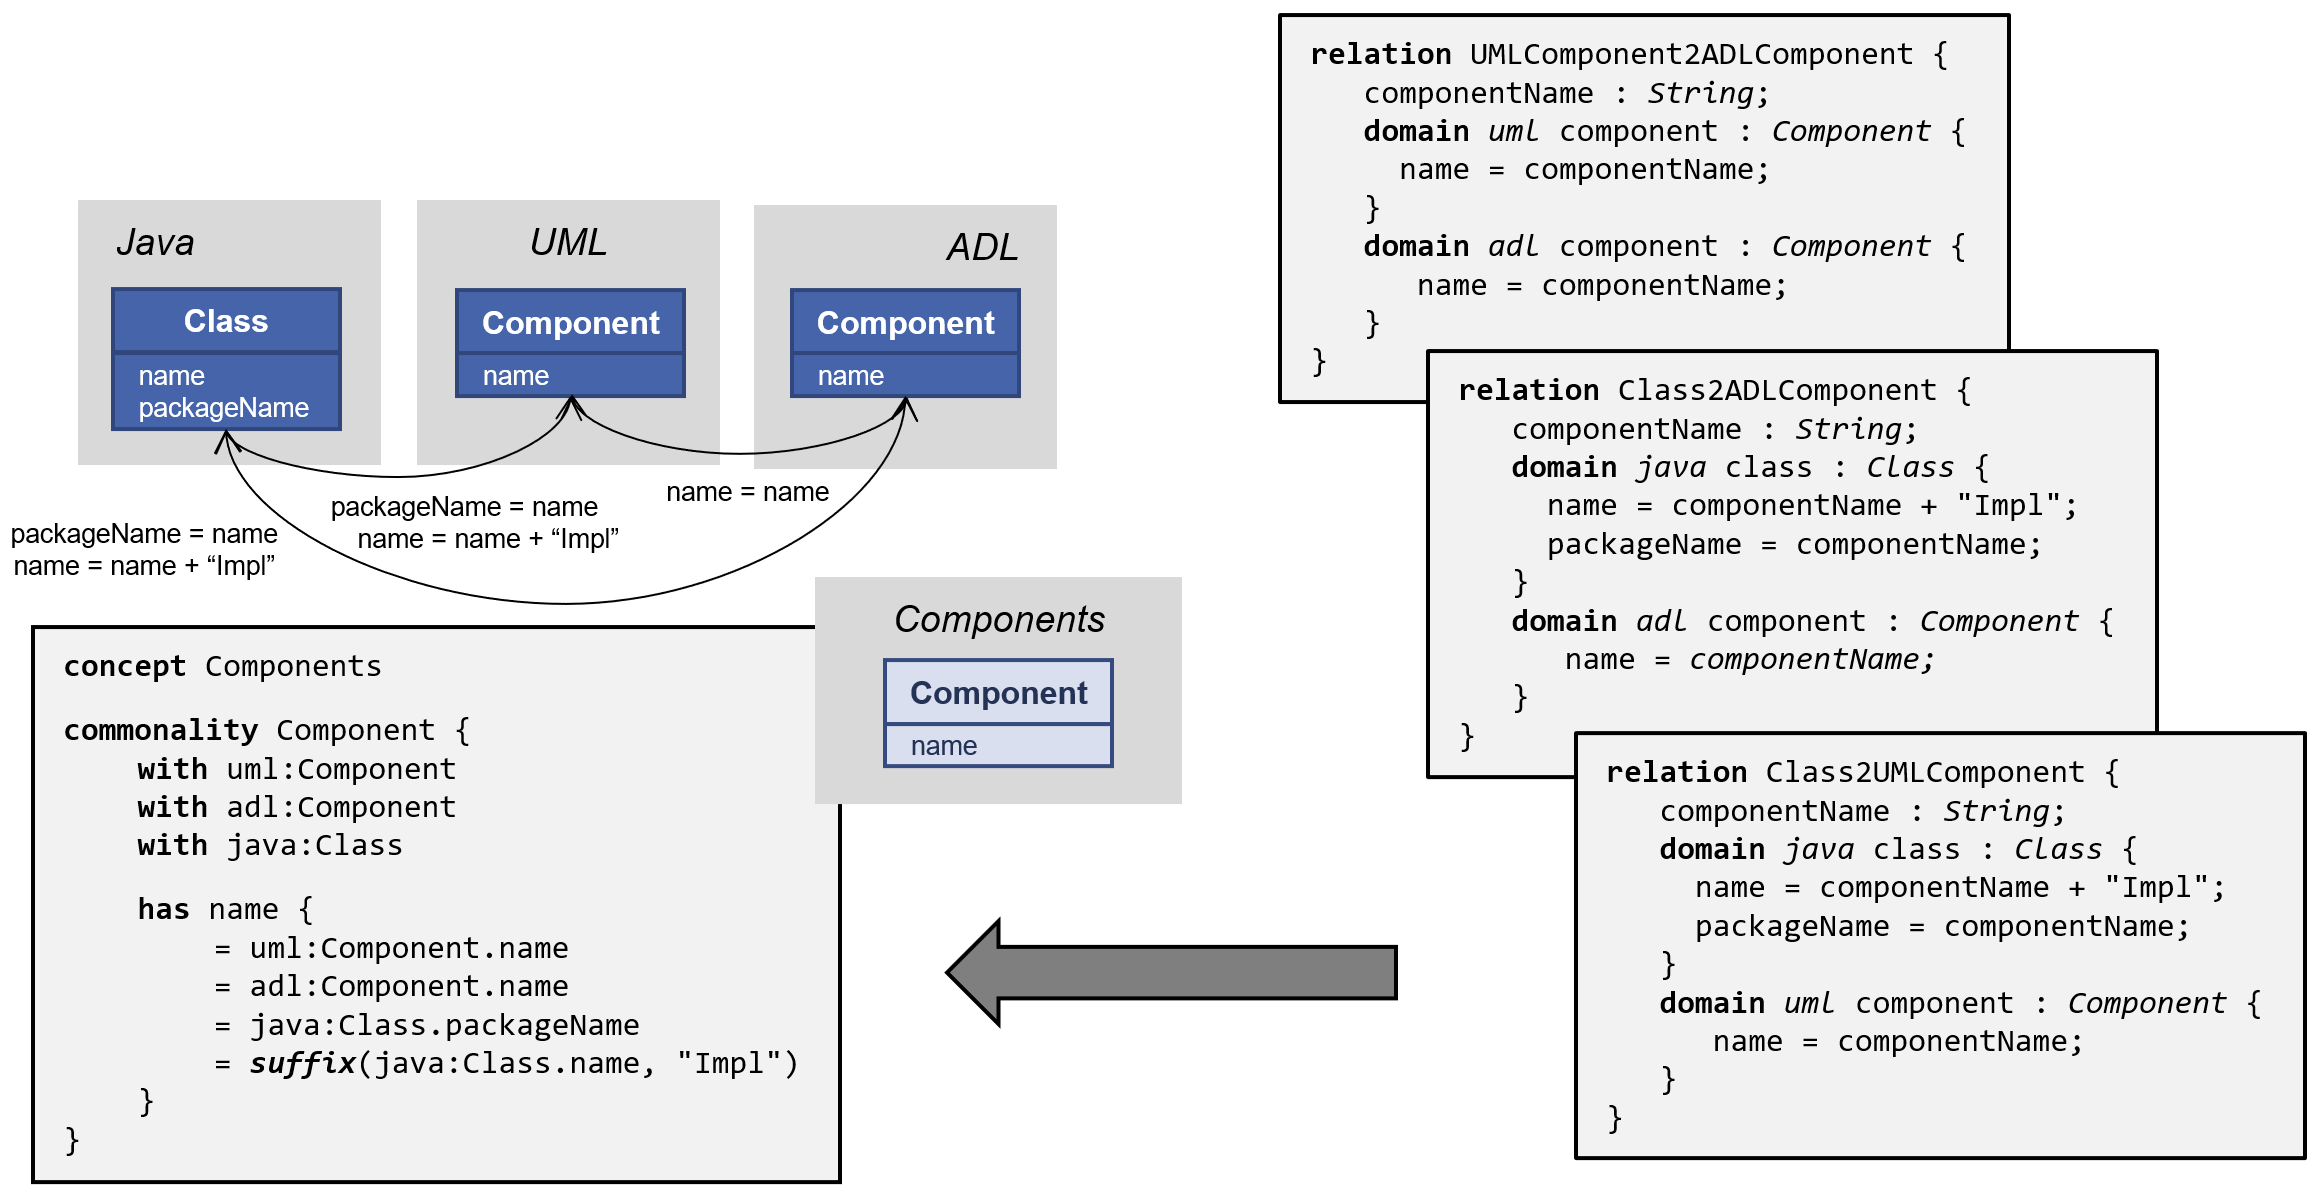
\includegraphics[width=\textwidth]{figures/quality/language/benefit_comprehensibility.png}
    \caption[Conciseness of \commonalities in comparison to \acrshort{QVTR}]{Example for consistency relations between classes and components expressed with \qvtr and the \commonalities approach.}
    \label{fig:language:conciseness_example}
\end{figure}

\mnote{\qvtr and \commonalities comparison example}
In \autoref{fig:language:conciseness_example}, we depict simplified consistency relations between components in \gls{PCM} and \gls{UML}, as well as classes in Java, together with a specification of these relations in \qvtr and the \commonalities language.
In contrast to our previous examples in \autoref{lst:language:class_example} and \autoref{lst:language:component_example}, the \commonalities specification does not define a hierarchy of \commonalities with two \conceptmetamodels for component-based and object-oriented design, but defines the Java manifestation within the component \commonality.
The example gives an impression of the expected conciseness of \commonalities specifications in comparison to ordinary, bidirectional specifications, due to which we expect benefits regarding comprehensibility and specification effort.

\mnote{Improving comprehensibility}
As a first benefit, we expect the \commonalities language to improve comprehensibility.
The language decomposes the specification of consistency along the \commonalities rather than along the transformations as with ordinary transformation languages.
In consequence, the information how a single common concept is represented in different metamodels is necessarily spread across several transformations if each transformation only relates two metamodels.
With \commonalities, this information is located at a single place, which is the specification of the according \commonality.
We expect this to improve the overall comprehensibility of how different elements in different metamodels sharing a common concept are related.
While a \commonalities specification improves compatibility anyway due to its likeliness of leading to a consistency relation tree, it can also make it easier for developers to get a global understanding of consistency, which would be necessary to avoid incompatibilities.
This is due to the reason that incompatibilities occur when different transformations relate the same elements in different ways, which becomes less likely if these different transformations are defined at one place, within the \commonality, such that developers responsible for other metamodels and thus further manifestations of that \commonality can easily understand the notion of consistency the other developers have.
\autoref{fig:language:conciseness_example} demonstrates how information about a component \commonality is represented at one place with the \commonalities language, whereas it is spread across three \qvtr transformations relating all pairs of metamodels.
As discussed in \autoref{chap:improvement:benefits:specification_effort}, the number of transformations increases even quadratically with the number of manifestations to keep consistent.
Finally, this is only a benefit of the \commonalities language, which realizes an internal specification of concepts (see \autoref{chap:language:design:internal_external}), because only such a realization decomposes the specification along the \commonalities.

\mnote{Reducing specification effort by \commonalities approach}
In \autoref{chap:improvement:benefits:specification_effort}, we have discussed the reduced specification effort of the \commonalities approach in general, when considering the scenario that a further metamodel shall be kept consistent.
Especially if the information this metamodel shares with other \concretemetamodels of an existing \commonalities specification is already represented by \commonalities, only the manifestation relations of the elements of the metamodel to be added to the existing \commonalities have to be defined.
In an ordinary transformation network, all pairwise relations of the metamodel to be added and the existing metamodels, with whom it shares common concepts, have to be defined, potentially leading to duplications and thus higher effort.

\mnote{Reducing specification effort by \commonalities language}
We have, however, also discussed that the effort for keeping instances of two metamodels consistent or, analogously, the initial effort for defining \commonalities for multiple metamodels by specifying the \commonalities for the first two of them can be high and, in particular, higher than defining ordinary transformations.
Two metamodels can be kept consistent by a single transformation, whereas a \commonalities specification requires an additional \conceptmetamodel and two transformations, one between each \concretemetamodel and that \conceptmetamodels, to keep them consistent.
The \commonalities language reduces the effort for specifying these three artifacts by the choice of an internal specification of concepts.
A single transformation rule for a consistency relation of a common concept is expressed by a \commonality, its manifestations and the specification of relevant features and their relation to the manifestations.
But instead of three places to define this information at, it is defined at the one place of the \commonality specification.
Although \autoref{fig:language:conciseness_example} only represents a single, simple example, it gives an impression of that a \commonalities specification, even concerning three rather than two manifestations to keep consistent, is not less concise than the expression of the according consistency relation in \qvtr.
This comparison implicitly assumes an intuitive comparison of conciseness in terms of lines of code.
It is, of course, an open question whether the specification effort actually correlates with such a metric and whether conciseness according to that metric is even given in further cases than the single one depicted here.
Nevertheless, we have argued indicators for expecting the benefit of reducing specification effort by the proposed language, but emphasize that its validation requires empirical studies in terms of controlled experiments with developers applying both approaches and measuring their effort in terms of necessary time to achieve an error-free solution.
We provide preliminary results of such an evaluation in \autoref{chap:commonalities_evaluation}.


%% OLD STRUCTURE WITH OPERATIONALIZATION AND BENEFITS IN OWN SECTIONS
% \section{Operationalization of Transformations}
% \label{chap:language:operationalization}

% \mnote{Operationalization according to \mappings language}
% In the previous section, we have discussed relevant elements for the \commonalities language and their semantics.
% We have also sketched an exemplary textual syntax, we which have also used for the prototypical implementation of the language.
% In \autoref{chap:language:design:artifacts_process}, we have already depicted that such a specification needs to be compiled to \conceptmetamodels and transformations between them an existing \concretemetamodels to be used as an ordinary transformation network.
% Since the semantics of relations defined between a \commonality and its manifestations is analogous to the semantics of bidirectional relations defined in the \mappings language~\cite[Chap.~7]{kramer2017a}, we refer to that detailed discussion for the operationalization of \commonalities specifications to transformations.

% \mnote{Essential compiler responsibilities}
% We still discuss essential responsibilities of the compiler process.
% First, we consider the compilation to the \reactionslanguage, which is part of the \vitruv framework, implements delta-based consistency preservation rules according to our formalism in \autoref{chap:correctness} and is the same language to which artifacts of the \mappings language compile.
% Then, we discuss how the scenarios of \commonality instantiation and deletion by means of matching manifestations, and of updates by means of operator execution are realized.

% \subsection{Compiling to \reactions}

% \mnote{Suitability of \reactions}
% The operationalization of \commonalities specifications requires the derivation of transformations and, in particular, their consistency preservation rules according to \autoref{def:consistencypreservationrule}.
% Thus, we need to derive rules that instantiate, delete or update \commonalities after changes to a manifestation, such that they are again consistent to the consistency relations implied by the manifestation relations defined in the \commonalities specification, and vice versa.
% The \reactionslanguage (see \autoref{chap:foundations:transformations:reactions}) allows the definition of \reactions and routines that restore consistency after changes.
% Each \reaction defines the type of change it reacts to and executes routines, which identify whether the consistency relation to which they preserve consistency is violated by that change and then execute actions to restore it.
% Since that kind of specification fits to the goals of the operationalization of \commonalities specifications, we described the operationalization to \reactions and have also implemented it in our prototype.
% An analogous operationalization has been developed for the \mapping language by \textcite[Sec. 7.7]{kramer2017a}.

% \mnote{\Reactions for each change type}
% The operationalization of \commonalities to \reactions requires that a \reaction is created for each change that may require the instantiation, deletion or update of a \commonality.
% Thus, for each \metaclass and each feature references within a \commonality, a \reaction for their changes has to be created.
% We discuss the details for the different scenarios of instantiation, deletion and update in the subsequent subsections.

% \mnote{Benefits of \reactions}
% A benefit of compiling to \reactions is that they have well-defined semantics~\cite[Sec. 6.7]{kramer2017a} and that they are proven complete and correct~\cite[Sec. 9.2.4 and 9.3]{kramer2017a}.
% This means that they are able to preserve consistency according to any possible consistency relation and that their execution actually actually preserves consistency to the consistency relation that is implied by the specified consistency preservation rule.
% Thus, the transformation language with which the manifestation relations of \commonalities are operationalized does especially not restrict expressiveness in any way.


% \subsection{Matching Manifestations}

% Conforms to instantiation (/deletion)

% \cite[Sec. 7.7.4]{kramer2017a}.
% Instantiation: \cite[Alg. 1]{kramer2017a}
% Deletion: \cite[Alg. 2]{kramer2017a}
% Feature update: \cite[Alg. 3]{kramer2017a}


% \subsection{Executing Operators}

% Conforms to update
% Operators are executed as soon as one of the used values (parameters) is changed
% Reuse mechanisms, libraries of operators


% \section{Expected Benefits}

% The \commonalities approached proposed in \autoref{chap:improvement} can provide several benefits compared to an ordinary network of transformations, especially in terms of mitigating the trade-off between correctness and reusability of the transformations.
% While that is a conceptual benefit that is given by construction of the approach and not only a claim that has to be validated, the expected benefits of a dedicated \commonalities language especially concern usability and applicability of the approach, which can be argued but also have to be empirically evaluated to provide further evidence.


% \subsection{Improving Comprehensibility}

% \begin{figure}
%     \centering
%     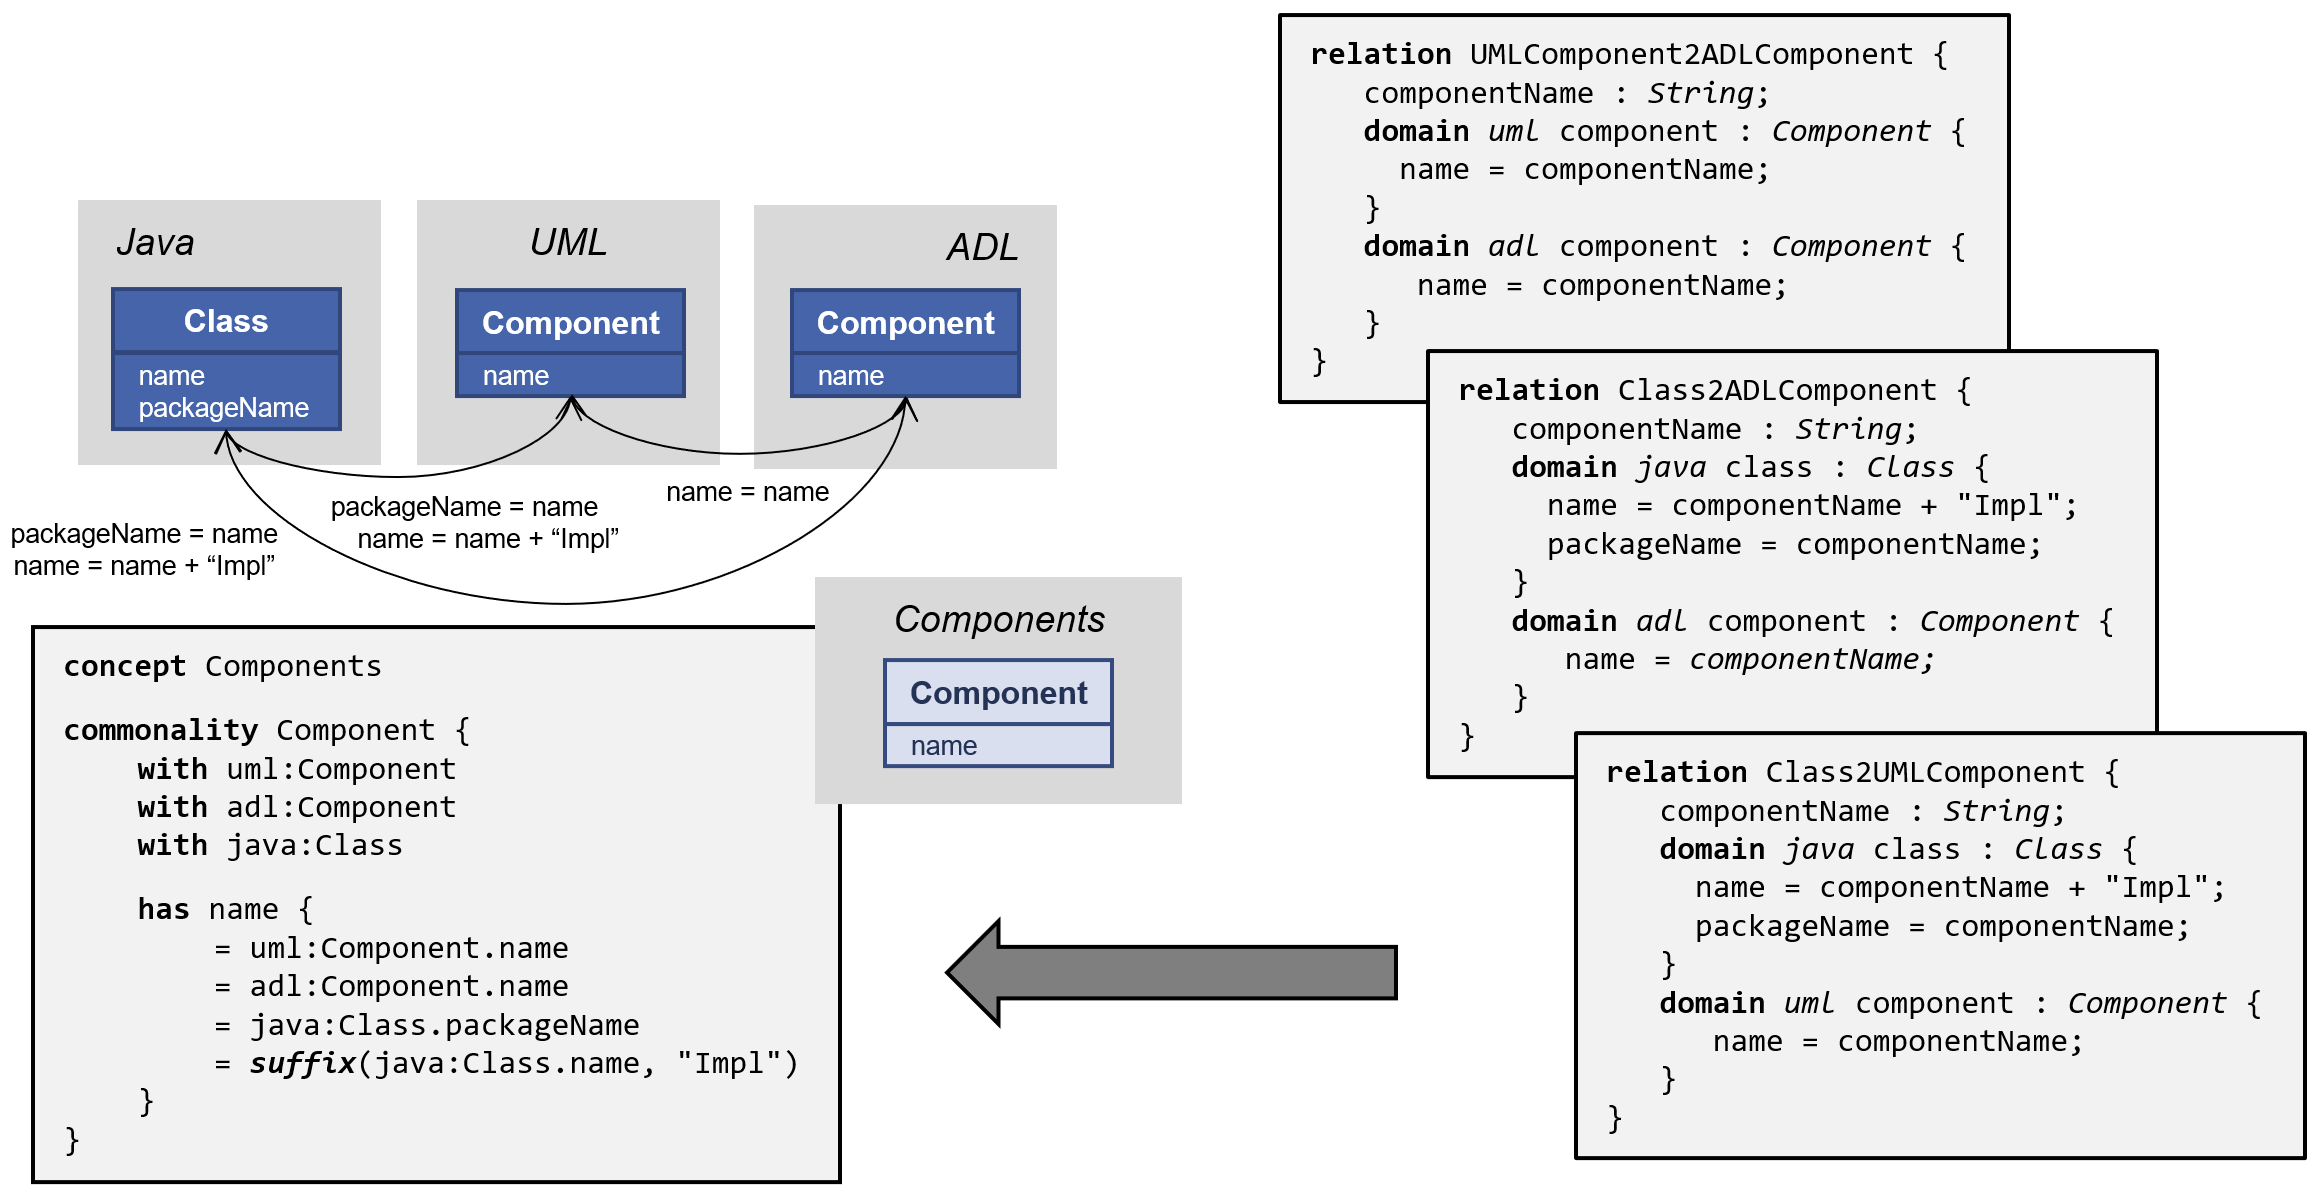
\includegraphics[width=\textwidth]{figures/quality/language/benefit_comprehensibility.png}
%     \caption[Benefit of \commonalities regarding comprehensibility]{Example for consistency relations between classes and components expressed with \qvtr and the \commonalities approach.}
%     \label{fig:language:benefit_comprehensibility}
% \end{figure}

% \subsection{Reducing Specification Effort}

% Further benefit: Specification effort, adding concrete metamodel, adapting commonality, easier with internal specification



% Implemented operators:
% * Attribute mappings operators: Mappings between attributes
% * Attribute reference operators: Mappings between attributes that serve as references, e.g., subpackages in UML and concept metamodel as explicit references whereas encoded as namespace attributes in classes in Java -> namespace attribute of Java class is mapped to package structure in UML
% * Condition operators

% \begin{copiedFrom}{VoSE}

% \section*{Language Description}

% As introduced before, our realization of the \commonalities language
% %for the previously explained \commonalities approach
% provides an internal concept definition and uses the \conceptmetamodels as additional metamodels in the operationalization.
% An example for the syntax of the \commonalities language is depicted in \autoref{lst:quality:commonalities_language_example}.

% % \begin{figure}
% %     \centering
% %     \todo{Potentially extend running example so that references are covered. At least, we do not have the package in the example}
% %     \includegraphics[width=\columnwidth]{figures/commonalities_language_example.PNG}
% %     \caption{An example for defining the common concept of components}
% %     \label{fig:commonalities_language_example}
% % \end{figure}

% % \lstinputlisting[language=commonalities, float, belowskip=-0.8 \baselineskip,
% %     caption={[Exemplary commonality for components]An exemplary specification of the \texttt{Component} \commonality between \gls{PCM}, UML and the object-oriented design concept in the \commonalities language},
% %     captionpos=b,
% %     label=lst:quality:commonalities_language_example,
% % ]{listings/quality/commonalities_language_example.lst}

% The language allows to define \conceptmetamodels by declaring \commonalities, each representing one commonality between different manifestations, such as the \texttt{Component} \commonality in our example.
% Relations between the \conceptmetamodels and their manifestations are supposed to be specified \emph{declaratively}.
% %, which is realized as a \metaclass in the \conceptmetamodel.
% For every \commonality, the \metaclasses in the manifestations that realize them are specified.
% In the example, the \texttt{Component} in \gls{PCM} and the \texttt{Class} in the object-oriented design \conceptmetamodel are %defined as representations of
% related to the \texttt{Component} \commonality.
% In our language, a \commonality is realized by a \metaclass in the metamodel that is generated for a concept, so the \texttt{Component} \commonality is realized by a \texttt{Component} \metaclass.

% Within a \commonality, attributes and references can be defined, similar to an ordinary \metaclass.
% The relations of an attribute to the manifestation are declared directly at the attribute.
% In the example, a \texttt{name} attribute is specified, which maps to the name of the component in \gls{PCM} and the name appended with an \enquote{Impl} suffix in Java.
% The language %defined by \textcite{gleitze2017a} 
% provides several operators for attribute relations, apart from equality relations.
% The example depicts a prefix operator that allows to compose a String attribute.
% Such operators can be defined independently and added to the language dynamically.
% References can be defined comparably to attributes but can be enriched with a definition of containment relations.

% % Introduce the idea of \enquote{Concepts} and \enquote{Commonalities}, explain how attributes and references are mapped.
% % \todo{We have to align the definition of Concept, Commonality etc. in the paper with the implementation}

% The actually conceptualized and implemented language by \textcite{gleitze2017a} is far more sophisticated than the simple overview we provide here. 
% It supports different kinds of bidirectional operators for attribute mappings, containment specifications (so-called \emph{participations}), attribute checks as preconditions for \commonality instantiation, and more.

% \end{copiedFrom} % VoSE
